\documentclass{amsart}

\usepackage[notref,notcite]{showkeys}
\usepackage[style=authoryear,ibidtracker=false,uniquename=false,giveninits=true,terseinits=true,maxbibnames=5,backend=biber]{biblatex}
\usepackage{float}
\usepackage{graphicx}
\usepackage{todonotes}
\usepackage{subcaption}
\usepackage{amsmath}
\usepackage{amsthm}
\usepackage{amssymb}
\usepackage[foot]{amsaddr}
\usepackage[misc]{ifsym}
\usepackage{enumerate}

\renewbibmacro{in:}{}
\addbibresource{rnni_polynomial.bib}

\newtheorem{lemma}{Lemma}
\newtheorem{theorem}{Theorem}

\newcommand{\rnni}{\mathrm{RNNI}}
\newcommand{\findpath}{\textsc{FindPath}}
\newcommand{\mrca}{\mathrm{mrca}}
\newcommand{\rank}{\mathrm{rank}}
\newcommand{\nni}{\mathrm{NNI}}
\newcommand{\fp}{\mathrm{FP}}
\renewcommand{\O}{\mathcal O}

\graphicspath{{figures/}}


\title[Computing $\rnni$ distance]{Efficient algorithm for computing nearest neighbour interchange distance between ranked phylogenetic trees}
\date{\today}
\author{Lena Collienne\textsuperscript{1}}
\email{lena.collienne@postgrad.otago.ac.nz}
\address{\textsuperscript{1}Department of Computer Science, University of Otago, New Zealand}
\author{Alex Gavryushkin\textsuperscript{1, \Letter}}
\email{\textsuperscript{\Letter}alex@biods.org}


\begin{document}

\begin{abstract}
We present a quadratic algorithm to compute shortest paths, and hence the distance, between ranked phylogenetic trees under the ranked nearest neighbour interchange operation.
\end{abstract}


\maketitle

Things to introduce:

\begin{itemize}
\item Trees with the notion of an interval in a tree (if we want intervals), clusters, subtrees induced by clusters.
Think about notations such as $(T)_k$, $(C)_T$, or similar.
\item $\findpath$, including its time complexity.
\item Note that $\findpath$ is deterministic, that is, an interval and a move on the interval are uniquely determined (this is necessary to concentrate on the $v, w$ nodes in the proof of main theorem).
\end{itemize}

\begin{theorem}
The time complexity of computing the $\rnni$ distance between trees on $n$ leaves is $\O(n^2)$.
\end{theorem}

\proof
We prove this theorem by showing that for every pair of trees $T$ and $R$, the path computed by the $\findpath$ algorithm is a shortest $\rnni$ path.
We denote this path by $\fp(T, R)$ and its length by $|\fp(T, R)|$.

Assume to the contrary that $T$ and $R$ are two trees with a minimum possible distance $d(T, R)$ such that $d(T,R) \neq |\fp(T,R)|$, that is, $d(T,R) < |\fp(T,R)|$.
Let $T'$ be the first tree on a shortest $\rnni$ path from $T$ to $R$.
Then $d(T',R) = d(T, R) - 1$ and the distance between $T'$ and $R$ is strictly smaller than that between $T$ and $R$.
Hence $d(T', R) = |\fp(T',R)| < |\fp(T,R)| - 1$.
We finish the proof by showing that no trees satisfy this inequality.

Specifically, we will show that for all trees $T$, $R$, and $T'$ such that $T'$ is one $\rnni$ move away from $T$,
\begin{equation}
	|\fp(T',R)| \geq |\fp(T,R)| - 1
 	\label{eqn:iff_inequality}
\end{equation}

\begin{figure}[!hbt]
\centering
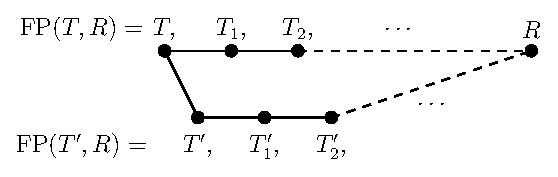
\includegraphics[width=0.6\textwidth]{proof_idea}
\vspace{12pt}
\caption{Trees $T, T'$ and $R$ contradicting inequality~(\ref{eqn:iff_inequality}) with $\fp(T,R) = [T,T_1,T_2, \ldots, R]$ and $\fp(T',R) = [T',T'_1,T'_2, \ldots, R]$}
\label{fig:proof_idea}
\end{figure}

Assume to the contrary that $T$ and $R$ are trees for which there exists $T'$ violating inequality~(\ref{eqn:iff_inequality}).
Out of all such pairs $T, R$ choose one with the path $\fp(T, R)$ as short as possible.
Denote $\fp(T,R)$ by $p$ and $\fp(T', R)$ by $p'$, and let $[(T)_t, (T)_{t+1}]$ be the interval in $T$ on which the $\rnni$ move connecting $T$ and $T'$ is performed.
As all clusters induced by nodes with rank $s \notin \{t, t+1\}$ in $T$ are induced by nodes of same rank $s$ in $T'$, $\rnni$ moves changing these clusters in $T$ can happen the same way on $T'$ and result in the same changes of clusters.
Let $C_k$ denote the cluster of $R$ whose most recent common ancestor is moved down on $p$ by the $\rnni$ move on $T$.
The first move on $p$ is on one of the intervals incident to node $(T)_t$ or $(T)_{t+1}$.
Indeed, if the rank of $(C_k)_T$, that is the most recent common ancestor of $C_k$ in $T$, was not in $\{t,t+1\}$, the move for decreasing the rank of $(C_k)_T$ on $p$ happens the same way on $p'$.
The existence of the pair of trees resulting from these moves on $T$ and $T'$, respectively, contradicts the assumption that we picked $T$ and $R$ with shortest $\fp(T,R)$ violating inequality~(\ref{eqn:iff_inequality}).

We will distinguish two cases, depending on whether $T$ and $T'$ are connected by an $\nni$ or a rank move.
For each of these we further distinguish all possible moves between $T$ and $T_1$.

Let $T$ and $T'$ be connected by an $\nni$ move as illustrated in Figure~\ref{fig:thm_fp_nni1}.
It follows that $((T)_{t+1},(T)_t)$ is an edge in $T$.
We denote the clusters induced by the children of $(T)_t$ by $A$ and $B$ and the cluster that is induced by the child of $(T)_{t+1}$ that is not $(T)_t$ by $C$, as it is depicted in Figure~\ref{fig:thm_fp_nni1}.
We assume without loss of generality that the $\nni$ move from $T$ to $T'$ exchanges the subtrees induced by clusters $A$ and $B$.
In the following we distinguish all moves possible between $T$ and $T_1$, that are moves on intervals incident to $(T)_t$ or $(T)_{t+1}$.

\begin{enumerate}[{Case} (1).]
\item If this $\nni$ move results in $T_1 = T'$, it is $|\fp(T',R)| = |\fp(T,R)| - 1$, which contradicts the assumption on the choice of $T'$.
If otherwise $T_1 \neq T'$, a new cluster $B \cup C$ is built in $T_1$.
Because $\fp(T,R)$ moves most recent common ancestors of clusters of $R$ down, it follows that the cluster $C_k$ that is currently considered by the algorithm contains taxa in $B$ and $C$.
From this observation it easily follows that $T_1$ follows $T'$ on $p'$ as well, because the same cluster $C_k$ is being considered on $\fp(T',R)$ in this step.
Therefore the remaining part of $p$ and $p'$ coincide, and it follows $|\fp(T',R)| = |\fp(T,R)|$, which again is a contradiction to the assumption $|\fp(T',R)| < |\fp(T,R)| - 1$.

\begin{figure}[!hbt]
\centering
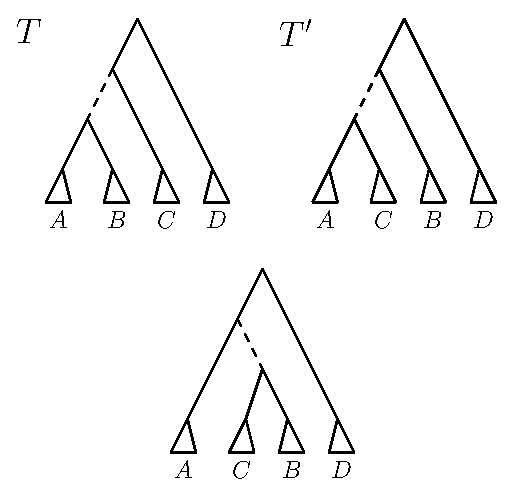
\includegraphics[width=0.4\textwidth]{thm_fp_nni1}
\vspace{12pt}
\caption{$\nni$ move between $T$ and $T'$ on the dashed edge $((T)_{t+1},(T)_t)$ and the third $\rnni$ neighbour resulting from a move on that edge.}
\label{fig:thm_fp_nni1}
\end{figure}

\item $\nni$ moves on edge $(u,v)$ above $(v,w)$

Notice that this is only possible if the interval above $(v,w)$ is an edge.
As it is depicted in the top of Figure~\ref{fig:thm_fp_nni2a}, there are two $\nni$ moves on $(u,v)$ possible that lead to different trees.
We stick to our notions of clusters $A,B,$ and $C$ as introduced above and additionally denote by $D$ the cluster induced by the child of $u$ that is not $v$.
An illustration of this can be found in Figure~\ref{fig:thm_fp_nni2a}.

\begin{figure}[H]
	\begin{subfigure}[b]{.45\textwidth}
		\centering
		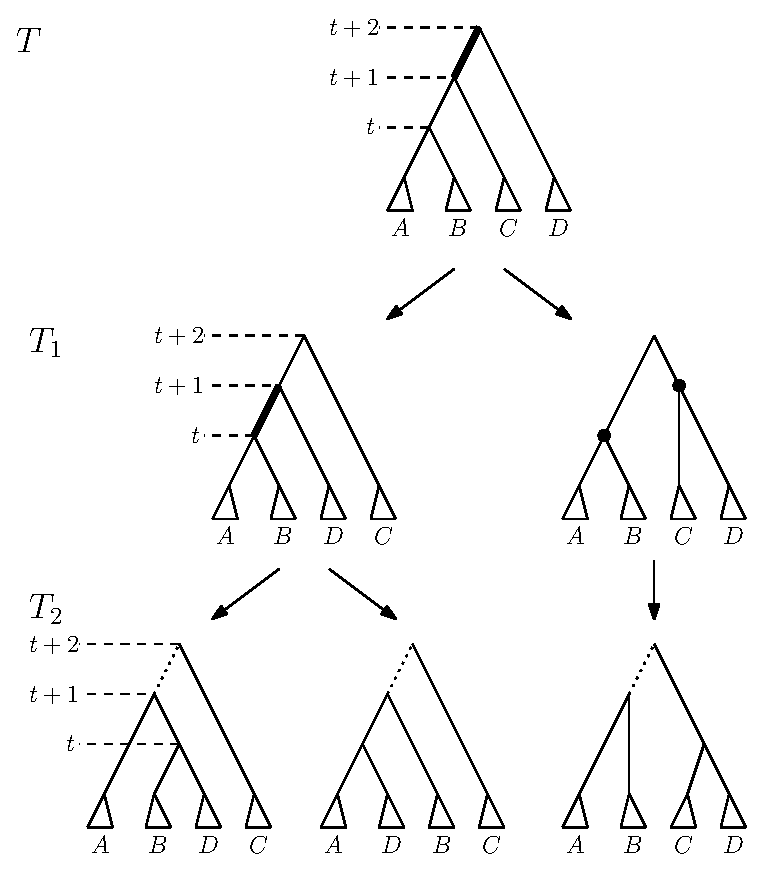
\includegraphics[width=0.9\linewidth]{thm_fp_nni2a.eps}
		\vspace{12pt}
		\caption{path $p$ following $T$}
		\label{fig:thm_fp_nni2a}
	\end{subfigure}
	\begin{subfigure}[b]{.45\textwidth}
		\centering
		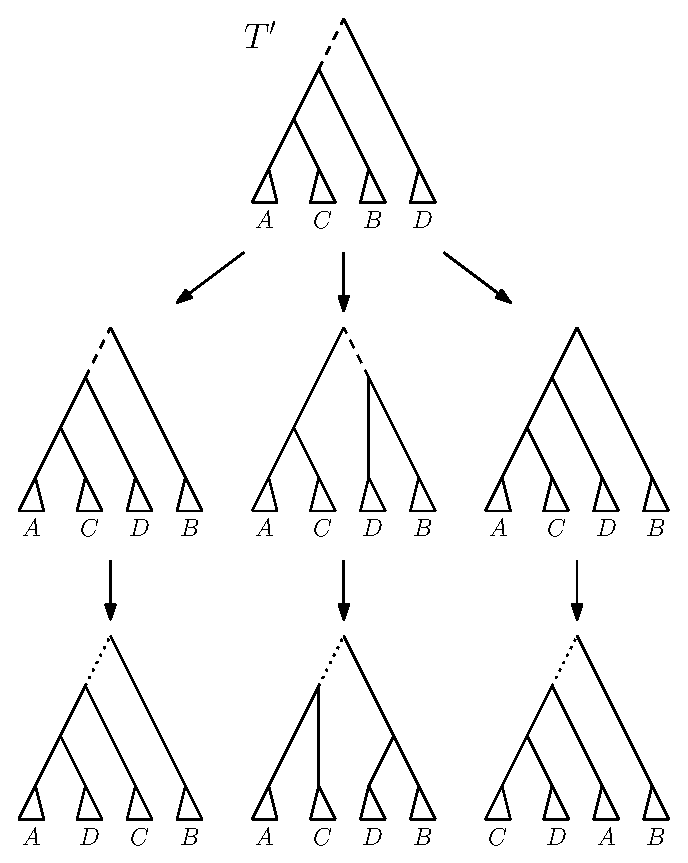
\includegraphics[width=0.9\linewidth]{thm_fp_nni2b.eps}
		\vspace{12pt}
		\caption{path $p'$ following $T'$}
		\label{fig:thm_fp_nni2b}
	\end{subfigure}
	\caption{Comparison of $p$ and $p'$ if there is an $\nni$ move on the edge $(u,v)$ above $(v,w)$ in $T$.
	The trees on the bottom are those following $T$ and $T'$ on $p$ and $p'$ after two $\rnni$ moves, respectively, depending on the cluster $C_k$ that is currently considered on $\findpath$:
	${C_k \subseteq A \cup D}$ on the left, ${C_k \subseteq B \cup D}$ in the middle, ${C_k \subseteq C \cup D}$ on the right.}
\end{figure}

We will now consider each of the $\nni$ moves that are possible between $T$ and $T_1$ separately.
If $T_1$ is the tree at the top left of Figure~\ref{fig:thm_fp_nni2a}, which results from $T$ by exchanging the subtrees induced by $C$ and $D$, the cluster $C_k$ that is moved down by $\findpath$ is either a subset of $A \cup B \cup D$, $A \cup D$ or $B \cup D$.

\begin{enumerate}
	\item If $C_k$ contains elements of all three clusters $A, B$ and $D$, then $C_{k-1} = A \cup B$ as the two clusters of $R$ that join to $C_k$ must already be present in $T$.
		\todo{Is this clear?}
		It follows that on $p'$ there is a move that moves the most recent common ancestor of $C_{k-1} = A \cup B$ down right before $C_k$ is considered, because $\findpath$ considers the cluster $C_{k-1}$ before cluster $C_k$.
		As a result the tree following $T'$ on $p'$ is $T$, contradicting $|\fp(T',R)| < |\fp(T,R)| - 1$.
	\item If $C_k \subseteq A \cup D$, the move on $T_1$ on $p$ moves $(C_k)_{T_1}$ further down by exchanging $B$ and $D$, resulting in a tree as depicted in the bottom left of Figure~\ref{fig:thm_fp_nni2a}.
		\todo{make sure this notion of mrca is introduced somewhere (if we really need it)}
		As the most recent common ancestor of the same cluster $C_k \subseteq A \cup D$ moves down on $p'$, the two moves following $T'$ exchange the subtree induced by $D$ down by exchanging it with its neighbours $B$ and $C$ as depicted on the left of Figure~\ref{fig:thm_fp_nni2b}.
		The trees on $p$ and $p'$ after these two moves following $T$ and $T'$, respectively, only differ by one edge (dotted edges in the trees at the bottom left of Figures~\ref{fig:thm_fp_nni2a} and~\ref{fig:thm_fp_nni2b}).
		This and the fact that $\findpath$ computes paths from these trees to $R$ that are shorter than $p$ contradicts the assumption that $\fp(T,R)$ has minimum length among all $\findpath$ paths between pairs of trees fulfilling inequality~\ref{eqn:iff_inequality}.
		\todo{I think we need the assumption that $|\fp(T,R)|$ is minimal here.}
	\item
		If $C_k \subseteq B \cup D$, the two $\rnni$ moves following $T$ and $T'$ on $p$ and $p'$, respectively, end up in the trees depicted in the tree in the middle at the bottom of Figures~\ref{fig:thm_fp_nni2a} and \ref{fig:thm_fp_nni2b}, analogous to the previous case.
		As in the previous case, these trees coincide in all but one interval (dotted edges in the figure), which again contradicts the assumptions on $T$ and $R$.
\end{enumerate}

If the $\nni$ move on $(u,v)$ results in a tree $T_1$ containing a subtree $C \cup D$ as illustrated on the top right of Figure~\ref{fig:thm_fp_nni2a}, it is $C_k \subseteq C \cup D$.
If $(C_k)_T$ does not move further down on $p$, it follows that $C_k = A \cup B$ is a cluster in $R$ and that before $C_k$ is considered on $p'$, the most recent common ancestor of $C_{k-1} = (A \cup B)_{T'}$ moves down by one $\rnni$ move.
Therefore $T$ follows $T'$ on $p'$, which contradicts $|\fp(T',R)| < |\fp(T,R)| - 1$.
If on the other side the rank of $(C_k)_T$ decreases by more than one after tree $T$ on $p$, the move on $T_1$ is a rank swap as depicted in the bottom right of Figure~\ref{fig:thm_fp_nni2a}.
The moves on $p'$ that decreases the rank of $(C_k)_{T'}$ are $\nni$ moves exchanging $D$ with $B$ and $A$, because it is $C_k \subseteq C \cup D$.
These moves are shown on the right of Figure~\ref{fig:thm_fp_nni2b}.
As above, the two trees resulting from the two moves following $T$ and $T'$ on $p$ and $p'$, respectively, coincide by all but one interval.
Therefore, we end up in the same contradiction as above.

\item Rank move on interval $[u,v]$ above $(v,w)$

Notice that this is only possible if $[u,v]$ is a rank interval.
If after the rank move, which increases the rank of $v$, there is a rank move on $T_1$ that increases the rank of $w$, the same rank moves happen on $p'$ and the trees after these two moves on $p$ and $p'$ coincide in all but one interval.
As previously, this contradicts the assumption that $T$ and $R$ are the closest trees where there is a $T' \in N_1(T)$ with $|\fp(T',R)| < |\fp(T,R)| - 1$.
If on the other side there is no such rank move on $T_1$, then the cluster $C_{k-1} = A \cup B$ induced by $w$ is a cluster in $R$ as well.
The tree following $T'$ on $p'$ is $T$ as it is the result of building this cluster in $T'$, which happens right before the cluster $C_k$ is being considered on $p'$.
This is due to the order in which $\findpath$ considers most recent common ancestors of clusters.
This contradicts $|\fp(T',R)| < |\fp(T,R)| - 1$.
\todo{add a figure for this case}

\item $\rnni$ moves on interval below $[v,w]$

If there is a move on the interval below $[v,w]$, it is $C_k \subseteq A \cup B$.
In this case, the move following $T'$ on $p'$ exchanges $B$ and $C$ by an $\nni$ move first, because this moves the most recent common ancestor of $C_k \subseteq A \cup B$ down.
However, this transforms $T'$ into $T$, which contradicts $|\fp(T',R)| < |\fp(T,R)| - 1$.
\end{enumerate}

Let us now assume that there is a rank move between $T$ and $T'$ where nodes $v$ and $w$ inducing clusters $A$ and $B$ swap ranks as depicted at the top of Figure~\ref{fig:thm_fp_rank1}.
We will again consider the different moves from $T$ to $T_1$ that are possible on intervals adjacent to $[v,w]$.

\begin{figure}[!hbt]
\centering
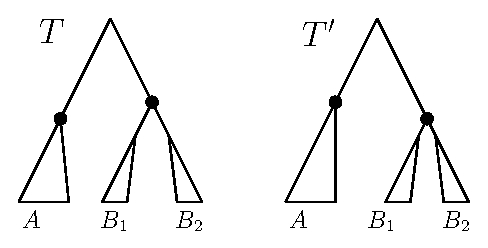
\includegraphics[width=0.4\textwidth]{thm_fp_rank1}
\vspace{12pt}
\caption{Rank move between $T$ and $T'$ on the interval given by the highlighted nodes, and an $\nni$ move on $T$ if the edge $(u,v)$ has length one.}
\label{fig:thm_fp_rank1}
\end{figure}

\begin{enumerate}
\item Rank move on $[v,w]$

The only possible move on $[v,w]$ on $T$ is a rank move resulting in $T_1 = T'$.
It follows $|\fp(T',R)| = |\fp(T,R)| - 1$, which obviously contradicts our assumption $|\fp(T',R)| < |\fp(T,R)| - 1$.

\item $\nni$ move on edge above $[v,w]$

Notice that this is only possible if the interval above $[v,w]$ is an edge $(u,v)$ of length one.
We are now going to distinguish the case that $u$ is the parent of $w$ from the case that it is not.
At first we assume that $u$ is parent of $w$.
It follows, that after the $\nni$ move on $(u,v)$, there is a new cluster containing $A$ and $B_1$, which is one of the subtrees that are children of $v$.
This move is depicted on the left of Figure~\ref{fig:thm_fp_rank1}.
If such a move happens the currently considered cluster $C_k$ must be subset of $A \cup B_1$, which means that $C_{k-1} = A$ is already at the same place in $T$ as in $R$.
Therefore, the move on $p'$ on $T'$ must be a rank swap leading to $T$, as $(A)_{T'}$ is moved to its correct position before $C_k$ is considered, which follows from how $\findpath$ works.
However, this means that $T$ is on the path $p'$ form $T'$ to $R$, which is a contradiction to $|\fp(T',R)| < |\fp(T,R)| - 1$

Let us now assume that $u$ is not the parent of $w$.
In this case the $\nni$ move builds a new cluster containing taxa of $B$ and of the cluster $C$ that is induced by the child of $u$ that is not $v$, as depicted in the top left of Figure~\ref{fig:thm_fp_rank2}.
It follows that $C_k \subseteq C \cup B_1$ where $B_1$ is one of the clusters that is induced by a child of $w$.
If there was no rank move on $T_1$ decreasing the rank of $(C_k)_{T_1}$ further, it must be $C_{k-1} = A$ meaning that $A$ is in the same position in $T$ as in $R$.
In this case the tree following $T'$ on $p'$ is be $T$ as $C_{k-1} = A$ moves to it's final position on $\findpath$ before $C_k$ is moved down.
However, this contradicts $|\fp(T',R)| < |\fp(T,R)| - 1$.
Let us now consider what happens if there is a rank move on $T_1$ that decreases the rank of $(C_k)_{T_1}$ on $p$.
This case is depicted on the left of Figure~\ref{fig:thm_fp_rank2}.
The moves happening on $p'$ are as follows.
As it is $C_k \subseteq C \cup B$, the rank of $(C_k)_{T'}$ decreases by a rank swap of $(C \cup B)_{T'}$ and $(A)_{T'}$ on $T'$ first and then an $\nni$ move exchanges $B_2$ and $C$, as it is depicted on the right in the same figure.
One can easily see that the two trees on $p$ and $p'$ that are two $\rnni$ moves apart from $T$ and $T'$, respectively, only differ by one interval.
Again, this is a contradiction to the fact that $T$ and $R$ are the trees with minimum distance for which we can find a $T' \in N_1(T)$ with $|\fp(T',R)| < |\fp(T,R)| - 1$.

\begin{figure}[!hbt]
	\centering
	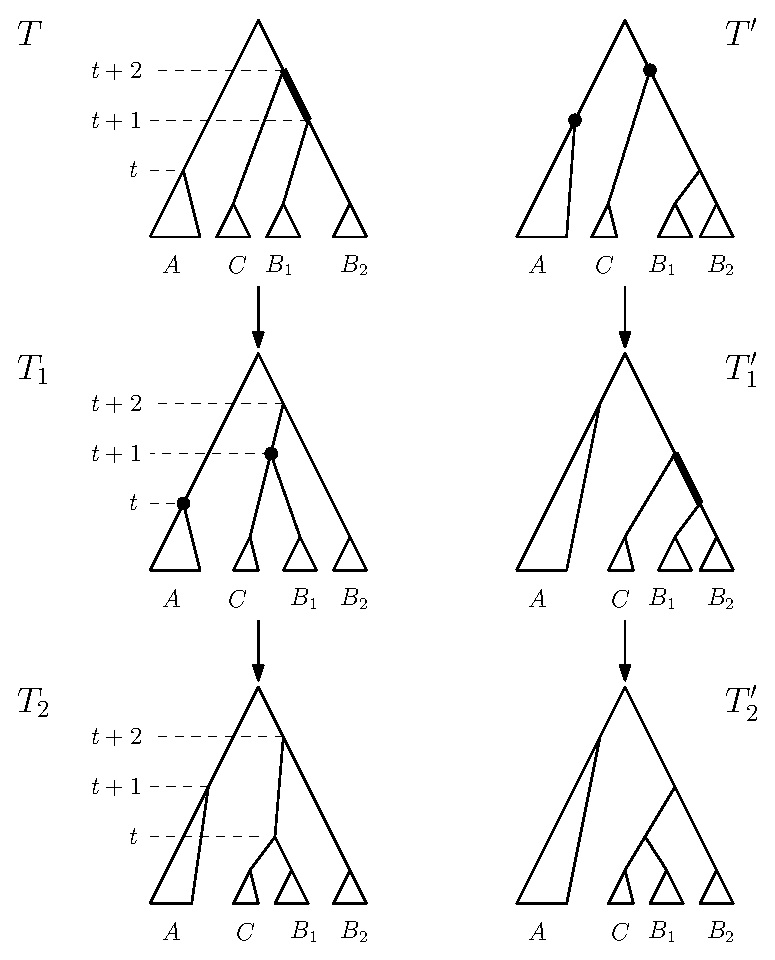
\includegraphics[width=0.4\textwidth]{thm_fp_rank2}
	\vspace{12pt}
	\caption{Comparison of $p$ (left) and $p'$ (right) if there is a rank move between $T$ and $T'$ and an $\nni$ move on the edge below the corresponding rank interval follows on $p$.}
	\label{fig:thm_fp_rank2}
\end{figure}

\item Rank move on interval above $[v,w]$

Notice that this is only possible if the interval above $[v,w]$ is a rank interval.
If there is a rank move increasing the rank of $v$, and no rank move increasing the rank of $w$ immediately afterwards, $C_k$ reaches it's final position in the tree $T_1$ on $p$ following $T$.
It follows that the cluster $A$ induced by $w$ in $T$ is the cluster $C_{k-1}$ in $R$.
This means that the move following $T'$ on $p'$ leads to $T$, as the node inducing $A$ moves down before $C_k$ is considered on $\findpath$.
This contradicts $|\fp(T',R)| < |\fp(T,R)| - 1$.
If on the other side the rank swap on $T$ is directly followed by a rank swap increasing the rank of $w$, such rank swaps happen on $p'$ as well and the trees following $T$ and $T'$ after two $\rnni$ moves on $p$ and $p'$, respectively, coincide in all but one interval.
This is again a contradiction to our choice of $T$ and $R$.

\item $\rnni$ moves on interval below $[v,w]$

If there is a move on the interval below $[v,w]$, it follows that $\findpath$ moves $C_k \subseteq A$ down where $A$ is the cluster induced by $w$.
For decreasing the rank of the most recent common ancestor of $C_k \subseteq A$ in $T'$, the move on $T'$ must be a rank swap that results in $T$, contradicting  $|\fp(T',R)| < |\fp(T,R)| - 1$.
\end{enumerate}

We can conclude that in any of the above cases we end up in a contradiction, proving that a tree $T'$ with $|\fp(T',R)| < |\fp(T,R)| - 1$ does not exist in $N_1(T)$.
Therefore we can follow that $|\fp(T',R)| \geq |\fp(T,R)| -1$ for all $T' \in N_1(T)$.
\endproof

\end{document}
